\section{Injection and removal of tritiated methane}

Two CH$_3$T sources with total activities of 3 Bq and 200 Bq were prepared for use in LUX. Each source is contained in a 2.25 liter stainless steel bottle and is mixed with 2 atmospheres of LUX-quality purified xenon. The xenon acts as a carrier gas to extract the source from the bottle. The CH$_3$T was synthesized for LUX by Moravek Biochemical \cite{moravek} at a specific activity of 5 milliCurie per millimol.

The injection system is shown in Fig. \ref{fig:plumbing}. A fraction of the source bottle activity may be extracted allowing the carrier gas to expand into one or more expansion volumes consisting of various sections of evacuated tubing. The amount of extracted activity is controlled by selecting an expansion volume of appropriate size. A methane purifier (SAES model MC1-905F) located between the source bottle and the expansion volume ensures that only CH$_3$T and noble gases are allowed to enter the system. The extracted activity is then injected into the TPC by diverting a small portion of the LUX xenon gas flow through the expansion volumes. 

\begin{figure}[H]\centering
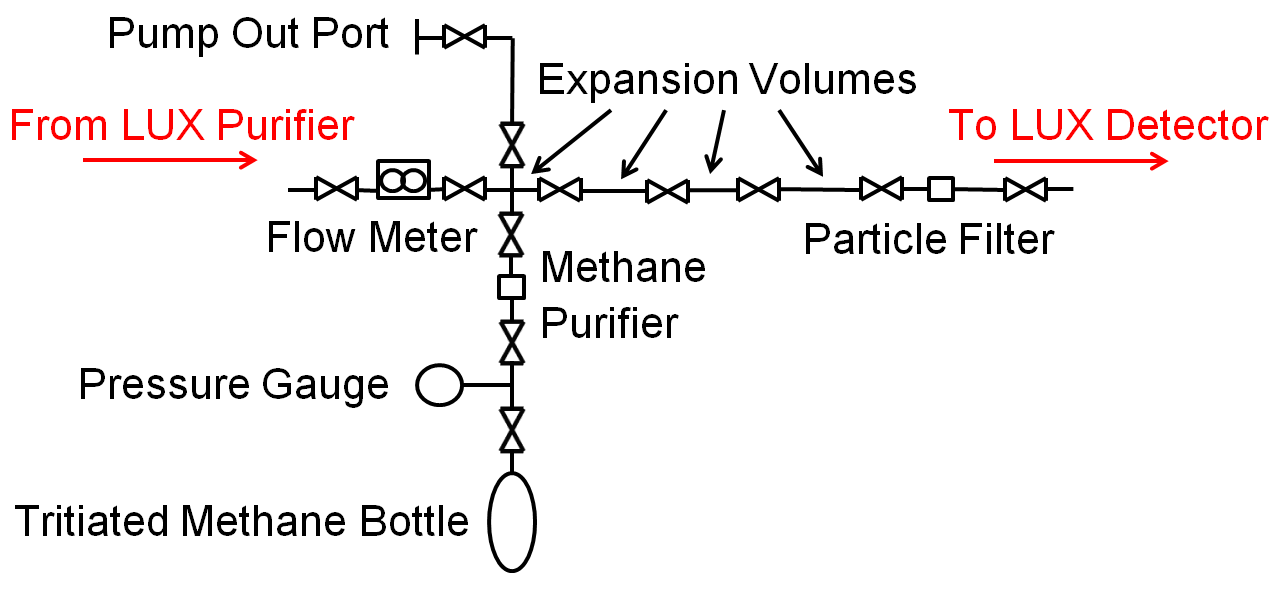
\includegraphics[width=80mm]{fig/TritiumPlumbing.png}
\caption{Plumbing diagram of the CH$_3$T injection system for LUX. CH$_3$T is injected downstream of the LUX xenon purifier so that it passes through the detector once prior to being removed.  Red arrows indicate the direction of flow.}
\label{fig:plumbing}
\end{figure}

The CH$_3$T appears in the TPC soon after the injection is performed and is removed via the normal action of the LUX xenon purification system, which operates without interruption during the entire procedure. Its centerpiece is a hot zirconium getter (SAES model PS4-MT15-R1) which acts upon gaseous xenon and removes all non-noble species including methane. The xenon gas flow is driven by a diaphragm pump and is facilitated by an efficient two-phase heat exchanger to effect the liquid-gas phase change \cite{two phase_hx}. The xenon flows in a continuous and perpetual circuit between the TPC and the getter at a rate of 27 SLPM. 

Prior to the first injection of CH$_3$T activity, we first confirmed that the LUX getter unit was capable of efficient methane removal by injecting  $\sim$1 ppm (part-per-million) of natural methane (CH$_4$) into LUX. As shown in Fig. \ref{fig:ch4_removal}, the CH$_4$ concentration in the gas was observed over the next several days using a mass spectrometer. The CH$_4$ concentration was observed to decrease exponentially with a time constant of 5.9 $\pm 0.07$ hours. The one-pass efficiency of the getter for CH$_4$ was measured to be 97\% under the LUX flow and temperature conditions by sampling the gas before and after the getter. 

On August 8, 2013, an initial injection of 20 mBq of CH$_3$T was performed, followed five days later by an injection of 800 mBq.
The count rate of fiducial single-scatter events with S1 less than 150 phe during this time period is shown as a function of time in Fig. \ref{fig:ch3t_removal}. The CH$_3$T activity is clearly observed. For both injections the activity was removed with a six-hour exponential time constant similar to that observed in the CH$_4$ injection. It is interesting that the purification time constant is considerably shorter than the naive volume turn-over time of LUX (about 41 hours for 370 kg of xenon at a gas flow rate of 27 SLPM).  The origin of short purification time remains under investigation.

\begin{figure}[h!]\centering
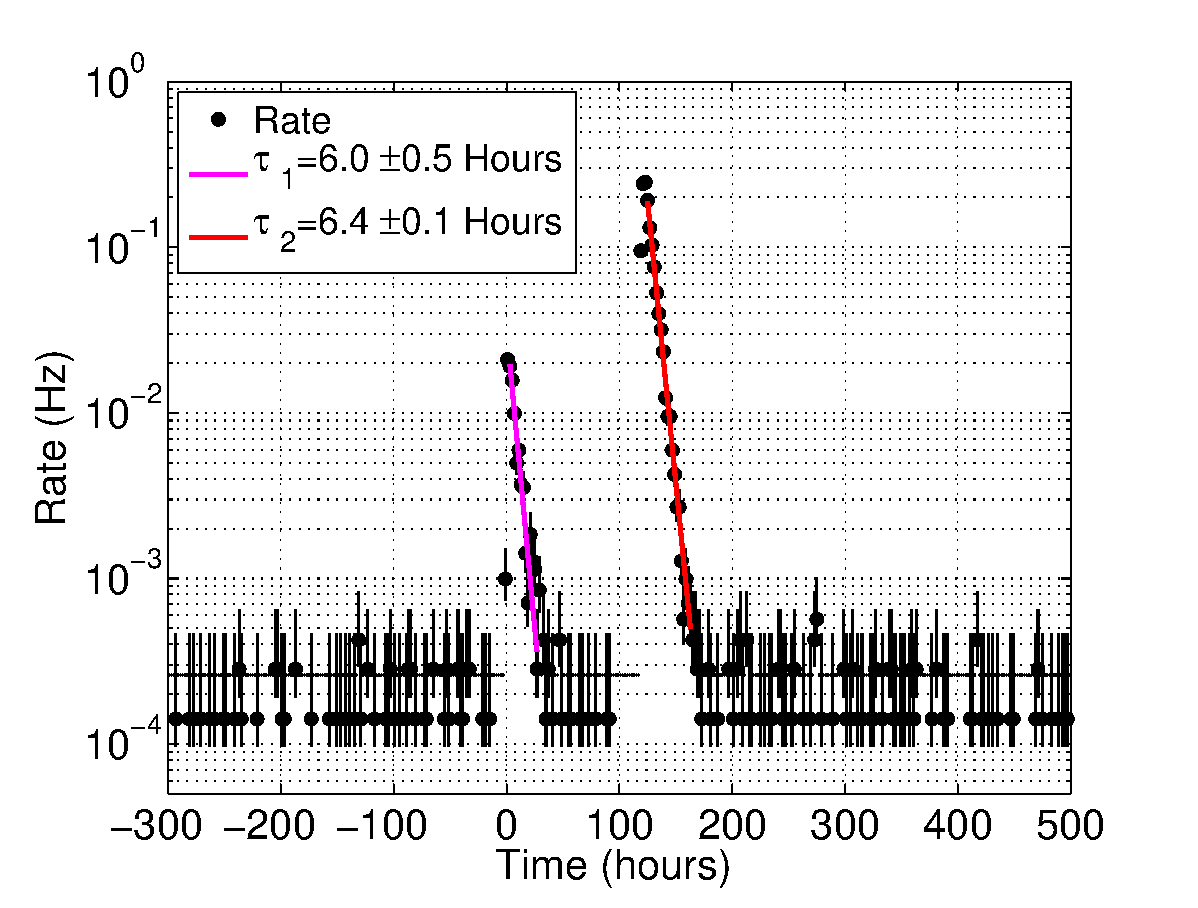
\includegraphics[width=80mm]{fig/CH3T_Rate_fid_150_Run03_Tritium_Rate.eps}
%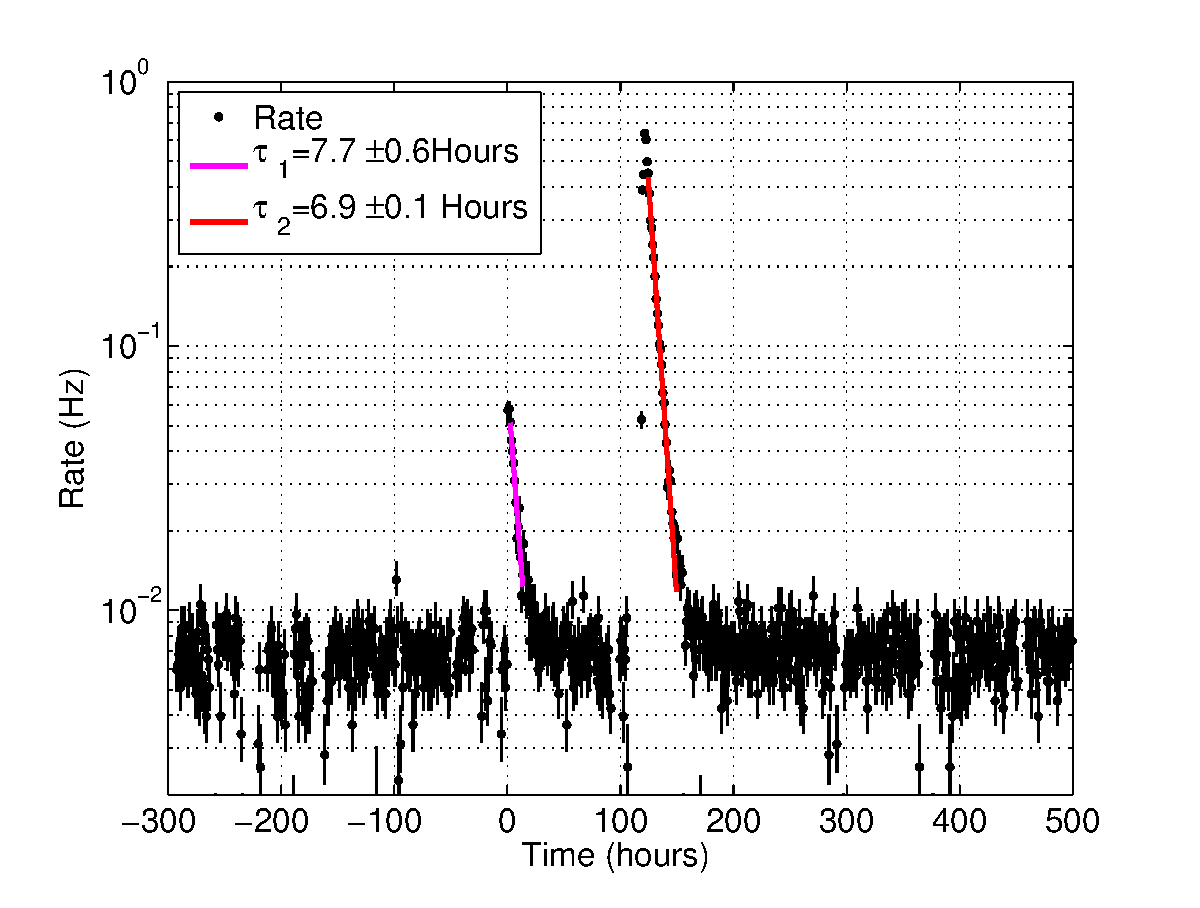
\includegraphics[width=60mm]{CH3T_Rate_Nofid_150_Run03_Tritium_Rate}
\caption{Left: Rate of single scatter events with S1 below 150 Phe in the fiducial volume during the August 2013 CH$_3$T injections. 150 Phe in S1 is about 18.6 $\rm keV{ee}$, the endpoint of the tritium beta spectrum. The magenta and red curves are exponential fits to the activity vs time.}
\label{fig:ch3t_removal}
\end{figure}

The location of a the CH$_3$T events from the first injection is shown in Fig. \ref{fig:event_location}. As expected the events are uniform within the detector volume.
 
\begin{figure}[h!]\centering
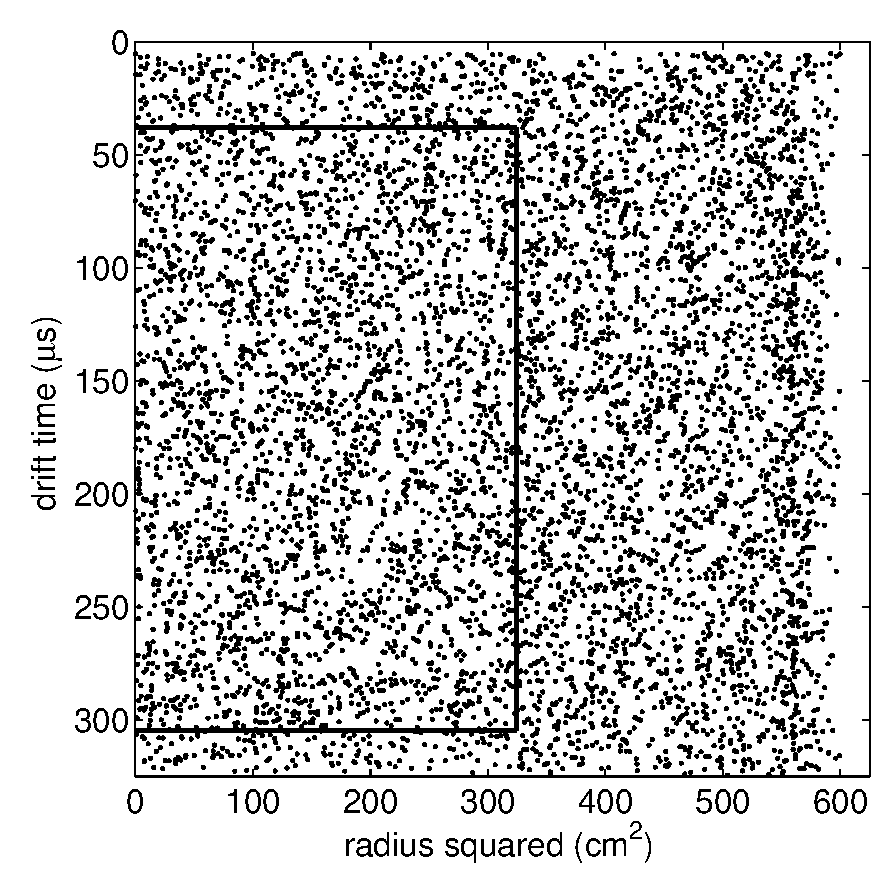
\includegraphics[width=80mm]{fig/CH3T_RZ_scatter_lux10_20130812T1546.eps}
\caption{The location of events in drift time vs. detector radius squared for the first CH$_3$T injection. The drift time is a proxy for the $z$ coordinate of the event. The solid black line represents the fiducial volume used in \cite{luxresults}.}
\label{fig:event_location}
\end{figure}





